\section{Kết quả thực nghiệm}
\subsection{Mô hình ban đầu}

\subsubsection{Thiết lập thực nghiệm}
\begin{itemize}
    \item \textbf{Dữ liệu sử dụng:} Dữ liệu được thu thập trực tiếp từ phần cứng và được tổng hợp lại đến khi đủ 1,680 dữ liệu thì đưa vào mô hình dự đoán.
    \item \textbf{Cấu hình mô hình:}
    \begin{itemize}
        \item Mô hình LSTM với kiến trúc gồm một lớp LSTM (128 đơn vị), một lớp Dropout (tỷ lệ 50\%), và hai lớp Dense (64 đơn vị và đầu ra 5 lớp).
        \item Hàm mất mát: \texttt{categorical\_crossentropy}.
        \item Trình tối ưu: Adam.
        \item Số epoch: 300.
        \item Kích thước batch: 4,500.
    \end{itemize}
\end{itemize}

\subsubsection{Kết quả huấn luyện và kiểm tra}
\begin{itemize}
    \item \textbf{Độ chính xác trên tập huấn luyện:} Khoảng 70\%, cho thấy mô hình đã học được một phần các đặc trưng từ dữ liệu.
    \item \textbf{Độ chính xác trên tập kiểm tra:} Khoảng 70\%, phản ánh mô hình có khả năng tổng quát hóa ở mức trung bình.
\end{itemize}

\subsubsection{Kết quả dự đoán thời gian thực}
\begin{figure}[H]
    \centering
    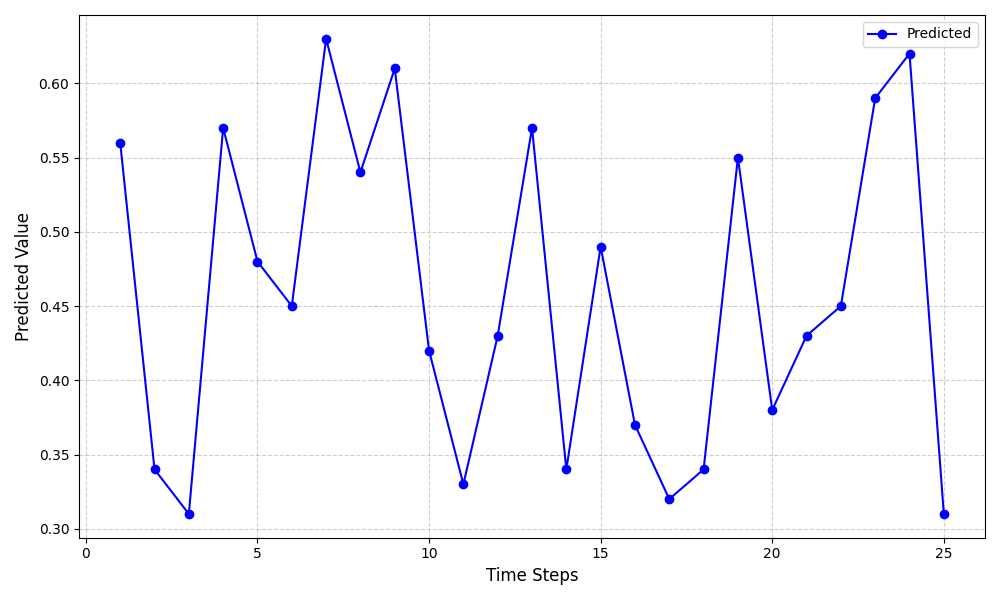
\includegraphics[width=\textwidth,height=\textheight,keepaspectratio]{Images/Experimental results/model.png}
    \caption{Kết quả thực nghiệm mô hình}
    \label{fig:enter-label}
\end{figure}
\begin{itemize}
    \item Khi thử nghiệm trên dữ liệu realtime từ các cảm biến, kết quả dự đoán của mô hình cho từng nhãn dao động trong khoảng từ 0.3 đến 0.6.
    \item Với ngưỡng phân loại đúng là trên 0.5, nhiều dự đoán không vượt qua ngưỡng này, dẫn đến kết quả không đáng tin cậy trong thực tế.
\end{itemize}

\subsubsection{Phân tích kết quả}
\begin{itemize}
    \item \textbf{Mô hình hoạt động tốt hơn trên dữ liệu tĩnh:}
    \begin{itemize}
        \item Độ chính xác trên tập kiểm tra cho thấy mô hình có khả năng học và phân loại ở mức cơ bản khi sử dụng dữ liệu tĩnh.
        \item Tuy nhiên, trên dữ liệu realtime, mô hình không thể duy trì hiệu suất, đặc biệt khi các tín hiệu có nhiễu hoặc thay đổi không đồng nhất.
    \end{itemize}

    \item \textbf{Khả năng phân biệt kém:}
    \begin{itemize}
        \item Kết quả dự đoán cho thấy nhiều nhãn có xác suất gần nhau, dao động quanh ngưỡng 0.5, thể hiện mô hình không tự tin trong việc phân loại.
        \item Điều này có thể do dữ liệu huấn luyện chưa đủ phong phú hoặc chưa đại diện tốt cho các trường hợp thực tế.
    \end{itemize}

    \item \textbf{Ảnh hưởng của dữ liệu nhiễu:}
    \begin{itemize}
        \item Trong môi trường thực tế, các yếu tố như nhiễu tín hiệu, dao động tay người dùng, hoặc sự không nhất quán trong cử chỉ có thể khiến dữ liệu đầu vào khác xa so với dữ liệu huấn luyện, làm giảm hiệu quả của mô hình.
    \end{itemize}
\end{itemize}

\subsection{Áp dụng cửa sổ trượt (Sliding Window)}

Kỹ thuật cửa sổ trượt (sliding window) đã được tích hợp và thử nghiệm trong hệ thống nhận diện cử chỉ thời gian thực. Đây là một phương pháp quan trọng giúp cải thiện độ chính xác dự đoán bằng cách chia nhỏ dữ liệu đầu vào thành các đoạn có độ dài cố định và xử lý tuần tự từng đoạn, tạo điều kiện cho mô hình học máy phân tích sâu hơn các chuỗi dữ liệu liên tục. Trong mục này, kết quả thực nghiệm của kỹ thuật sliding window được trình bày thông qua việc so sánh độ chính xác dự đoán và thời gian xử lý khi thay đổi kích thước cửa sổ.

\begin{figure}[H]
    \centering
    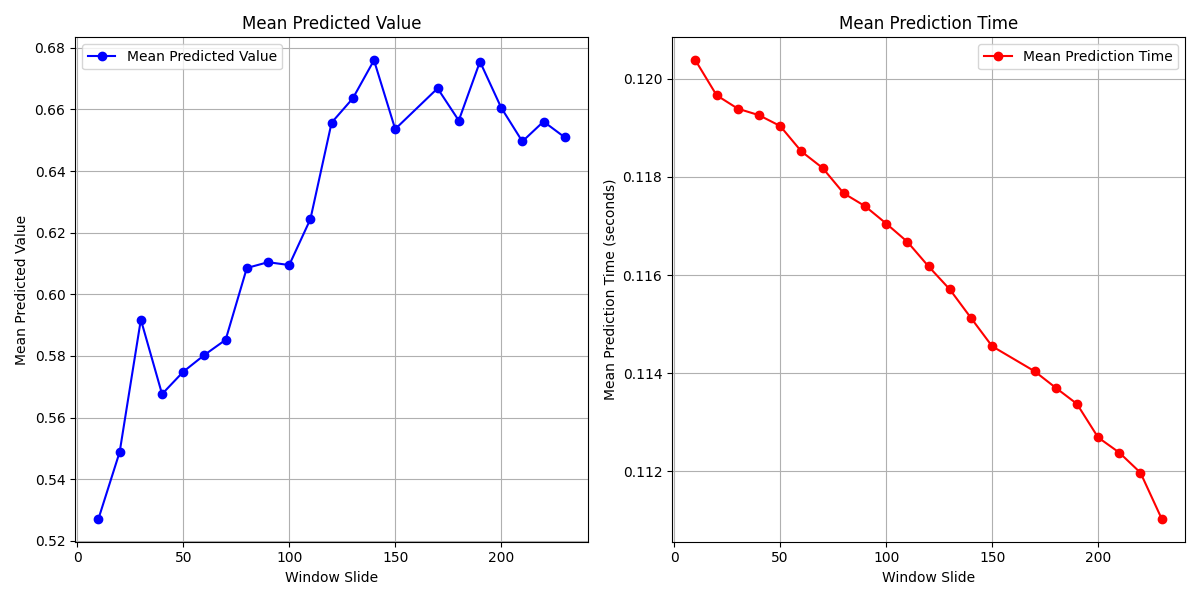
\includegraphics[width=\textwidth,height=\textheight,keepaspectratio]{Images/Experimental results/Sliding Window.png}
    \caption{Kết quả dự đoán và thời gian trung bình ứng với các giá trị sliding window}
    \label{fig:enter-label}
\end{figure}


\subsubsection{Độ chính xác dự đoán tăng theo kích thước cửa sổ}

Biểu đồ minh họa cho thấy rằng khi kích thước cửa sổ tăng dần từ 10 đến 230, độ chính xác dự đoán của hệ thống cũng tăng đáng kể. Cụ thể: 
\begin{itemize}
    \item Với kích thước cửa sổ nhỏ (10-50), giá trị độ chính xác trung bình dao động quanh mức 0.5. Kích thước nhỏ khiến hệ thống khó khai thác đầy đủ thông tin trong chuỗi dữ liệu, dẫn đến dự đoán kém ổn định.  
    \item Khi kích thước cửa sổ tăng lên (từ 100 đến 230), giá trị độ chính xác cải thiện đáng kể, đạt mức từ 0.6 đến gần 0.7. Điều này cho thấy rằng việc cung cấp nhiều dữ liệu hơn trong mỗi bước xử lý giúp mô hình nắm bắt tốt hơn các đặc điểm quan trọng trong chuỗi thời gian, qua đó tăng khả năng nhận diện chính xác.
\end{itemize}

\subsubsection{Thời gian dự đoán giảm nhẹ khi tăng kích thước cửa sổ}

Mặc dù kích thước cửa sổ tăng, thời gian xử lý mỗi lần dự đoán giảm nhẹ từ 0.12 giây xuống 0.11 giây. Điều này có thể được giải thích bởi hai yếu tố chính:
\begin{itemize}
    \item \textbf{Hiệu quả của mô hình học máy}: Mô hình được huấn luyện tối ưu với khả năng xử lý hiệu quả các chuỗi dữ liệu dài. 
    \item \textbf{Độ ổn định của bộ đệm dữ liệu}: Khi kích thước cửa sổ lớn, dữ liệu trong bộ đệm ít thay đổi thường xuyên hơn, giảm chi phí xử lý từng khung dữ liệu mới.
\end{itemize}
Mặc dù sự thay đổi về thời gian là không đáng kể, nhưng nó cho thấy rằng kỹ thuật sliding window không gây ra ảnh hưởng tiêu cực đến tốc độ xử lý thời gian thực của hệ thống.

\subsubsection{Kết luận}

Áp dụng kỹ thuật sliding window mang lại sự cải thiện đáng kể về độ chính xác dự đoán mà không ảnh hưởng tiêu cực đến tốc độ xử lý. Sự thay đổi kích thước cửa sổ giúp mô hình học máy thích nghi tốt hơn với dữ liệu đầu vào, nâng cao hiệu quả nhận diện trong các ứng dụng thời gian thực. Phương pháp này không chỉ đáp ứng được yêu cầu thực tiễn mà còn dễ dàng tinh chỉnh để phù hợp với các hệ thống khác nhau. 


\subsection{Khôi phục dữ liệu bị mất}

Trong quá trình thử nghiệm, dữ liệu thu thập từ phần cứng được gửi đến với tốc độ rất cao, khoảng 10ns/lần cho mỗi gói gồm 7 dữ liệu. Vì các lý do khách quan trong thực tế sẽ có hiện tượng mất dữ liệu trong khi truyền. Nhóm đã thực nghiệm nhiều lần và nhận thấy có hai trường hợp chính là mất ít dòng liên tục và nhiều dòng liên tục.

\subsubsection{Dữ liệu mất ít dòng (dưới 10 dòng)}

Khi dữ liệu mất ở mức độ nhỏ, chẳng hạn dưới 10 dòng (mỗi dòng chứa 7 giá trị dữ liệu), hệ thống có thể tận dụng dữ liệu gửi đến sau để bù đắp cho khoảng dữ liệu bị thiếu mà không cần áp dụng các phương pháp khôi phục dữ liệu phức tạp. Điều này mang lại hai lợi ích chính:
\begin{itemize}
    \item \textbf{Tăng tốc độ xử lý}: Tránh việc sử dụng các thuật toán phục hồi dữ liệu tốn thời gian, đặc biệt trong các ứng dụng thời gian thực.
    \item \textbf{Giữ ổn định hệ thống}: Dữ liệu được bù đắp bởi các giá trị liền kề, đảm bảo chuỗi dữ liệu tiếp tục được phân tích mà không bị gián đoạn.
\end{itemize}

Phương pháp này dựa trên giả định rằng sự mất dữ liệu trong khoảng thời gian ngắn không ảnh hưởng nghiêm trọng đến việc nhận diện cử chỉ, nhờ vào tính chất liên tục của chuỗi dữ liệu từ phần cứng.

\subsubsection{Dữ liệu mất nhiều dòng (trên 10 dòng)}

Khi hiện tượng mất dữ liệu xảy ra trên quy mô lớn hơn, các phương pháp khôi phục dữ liệu thông thường không còn đáng tin cậy. Điều này xuất phát từ việc thiếu thông tin ngữ cảnh để tái tạo chính xác chuỗi dữ liệu bị mất. Thay vào đó, một chiến lược hiệu quả hơn được đề xuất:
\begin{itemize}
    \item \textbf{Thiết lập cơ chế timeout}: Hệ thống sẽ theo dõi thời gian không nhận được dữ liệu từ phần cứng. Nếu vượt quá một khoảng thời gian định trước (timeout), hệ thống sẽ thực hiện việc khởi động lại quy trình nhận dữ liệu từ đầu.
    \item \textbf{Lợi ích của cơ chế timeout}:
    \begin{itemize}
        \item Đảm bảo rằng hệ thống không cố gắng xử lý các chuỗi dữ liệu không đầy đủ, tránh ảnh hưởng đến độ chính xác của mô hình.
        \item Đơn giản hóa quy trình xử lý, giảm thiểu chi phí tính toán so với các phương pháp phục hồi dữ liệu phức tạp.
    \end{itemize}
\end{itemize}

\subsubsection{Kết luận}

Với tốc độ gửi dữ liệu cao từ phần cứng, hệ thống có thể tự điều chỉnh để đối phó với hiện tượng mất dữ liệu mà không cần áp dụng các kỹ thuật khôi phục phức tạp. Đối với dữ liệu bị mất ít dòng, dữ liệu gửi đến sau có thể bù lại được, đảm bảo tính liên tục. Ngược lại, khi mất quá nhiều dữ liệu, cơ chế timeout sẽ đảm bảo rằng hệ thống nhận dữ liệu lại từ đầu, giữ vững tính ổn định và chính xác trong các ứng dụng thời gian thực.

Chiến lược này tối ưu hóa hiệu suất của hệ thống, giảm thiểu chi phí xử lý và phù hợp với yêu cầu của các ứng dụng nhận diện cử chỉ trong thực tế.




\subsection{1}
Data được thu thập sau đó được phân bổ với tỉ lệ 80-20, 80\% lượng data được sử dụng để train mô hình, 20\% được sử dụng để kiểm tra kết quả sau khi huấn luyện

Chúng ta không thể đánh giá kỹ năng của mô hình chỉ từ một lần đánh giá.
Nguyên nhân là mạng nơ-ron là ngẫu nhiên, có nghĩa là một cấu hình mô hình cụ thể khác nhau sẽ xuất hiện khi đào tạo cùng một cấu hình mô hình trên cùng một dữ liệu. Điều này là một đặc trưng của mạng, vì nó mang lại khả năng thích ứng cho mô hình, nhưng yêu cầu một quá trình đánh giá mô hình phức tạp hơn.

Chúng ta sẽ lặp lại việc đánh giá mô hình nhiều lần, sau đó tóm tắt hiệu suất của mô hình qua từng lần chạy đó. chúng ta có thể gọi hàm evaluate\_model() tổng cộng 5 lần.Điều này sẽ dẫn đến một tập hợp các điểm đánh giá mô hình cần được tóm tắt.'\\

\begin{lstlisting}
>#1: 90.058
>#2: 85.918
>#3: 90.974
>#4: 89.515
>#5: 90.159
>#6: 91.110
>#7: 89.718
>#8: 90.295
>#9: 89.447
>#10: 90.024

[90.05768578215134, 85.91788259246692, 90.97387173396675, 89.51476077366813, 90.15948422124194, 91.10960298608755, 89.71835765184933, 90.29521547336275, 89.44689514760775, 90.02375296912113]

Accuracy: 89.722% (+/-1.371)

\end{lstlisting}
Cuối cùng, mẫu các điểm đánh giá được in ra, tiếp theo là giá trị trung bình và độ lệch chuẩn. Chúng ta có thể thấy rằng mô hình đã hoạt động tốt, đạt được độ chính xác phân loại khoảng 89,7\% khi được huấn luyện trên dữ liệu thô, với độ lệch chuẩn là khoảng 1,3. Đây là một kết quả tốt ! 
\subsection{}

Dựa vào số động tác thực hiện và số lần mô hình xác định chính xác, cho thấy mô hình chỉ đạt kết quả khoảng 70\%: \\

Kết quả này được thực hiện như sau:\\
\begin{itemize}
    \item Một động tác được duy trì trong 2.4s bằng với số frame dữ liệu được gửi đến mô hình để dự đoán
    \item Thực hiện động tác với label 7 và 9 vì hai động tác này có data frame khá tương đồng nhau,  trong 1 phút bằng với 25 lần mô hình gửi đến model kết quả cho thấy chỉ dự đoán được 18 lần với label 7 và 17 lần với label 9
\end{itemize}
Những động tác có data frame khác biệt nhau ví dự như label 5 và label 0 cho ra kết quả khá chính xác, lên đến hơn 90\% dựa vào cách tính trên


